\section{Event Selection}
\label{sec:eventselection}

The event selection used is not optimized for any specific SUSY scenario.
It is based on small modifications to the dilepton event selections 
that we used in recently approved 
$WW$\cite{ww} and \ttbar\cite{ttbar} cross-section
analyses.  A quick summary of the event selection is:
\begin{itemize}
\item The event is required to pass the single $e$ or $\mu$  triggers.
\item Two isolated, same sign leptons ($ee$, $e\mu$, and $\mu\mu$). 
\item Leptons must have $P_T > 10$ GeV and at least one of them must have $P_T > 20$ GeV.
\item We veto the candidate lepton, if an extra lepton in the event, pairs with the candidate lepton
to form a $Z$ within the mass range between $76 < m_{\ell\ell} $ (GeV) $< 106$. This requirement is 
designed to reject $WZ$ events.
\item At least three L2L3 corrected caloJets with $P_T > 30$ GeV and $|\eta|< 2.4$.
\item The scalar sum of the $P_T$ of all jets passing the requirements above should be $>$ 200 GeV.
\item We require \met~$>$ 80 GeV. Track Corrected MET (tcMET) \cite{tcmet} is used as a measure for \met.
\end{itemize}
\noindent The details of the lepton and trigger selections are given below.

\subsection{Electron Selection}
\label{sec:electron}

\begin{itemize}
\item The electron ID is the ``e-gamma category based tight'', with small 
modifications to account for changes between CMSSW 1\_6\_X and 2\_2\_X; see Reference~\cite{ww} for details.
\item No muon candidate within $\Delta R < 0.1$.
\item $|d_0| < 200~\mu m$ (corrected for beamspot).
\item Iso $<$ 0.1, where Iso=Sum/Max(20 GeV, $P_T$), and Sum = tkIso + hcalIso +  Max(0 GeV, ecalIso - 2GeV).
All isolation sums are the standard sums used in release 2\_2\_X from the egamma group (cone of
0.4 for ecal, jurassic, rec-hit based; cone of 0.3 for tracker, and cone of 0.4 for hcal).
\item Conversion rejection~\cite{conversion} using tracks within cone of 0.3 of the candidate electron: 
\begin{itemize}
\item $|\Delta \cot\theta| < 0.02$; the difference between cotangent azimuthal angles of tracks parallel to 
each other.
\item $|d_{2d}| < 0.02$ cm; the two dimensional distance between points within nearest tracks.
\end{itemize} 
\end{itemize}

\subsection{Muon Selection}
\label{sec:muon}
\begin{itemize}
\item Must be a global muon {\bf and} a tracker muon~\cite{glbtrk}.
\item GlobalMuonPromptTight (global $\chi^2$/ndof$<$10)~\cite{muonid}.
\item At least 11 valid hits for the silicon track~\cite{muonid}.
\item $|d_0| < 200~\mu m$ (from silicon track, corrected for beamspot).
\item Minimum ionizing: EcalVetoEnergy $<$ 4 GeV and HcalVetoEnergy $<6$ GeV~\cite{vplusj}. 
\item Iso $<$ 0.1, where Iso=Sum/Max(20 GeV, $P_T$), and Sum = tkIso + hcalIso +  ecalIso.
All isolation sums are the standard sums stored in the muon object in release 2\_2\_X, and
are calculated in a cone of 0.3.
\end{itemize}

\subsection{Trigger Selection}
\label{sec:trigger}
We use inclusive lepton triggers with no isolation, $i.e.$, the logical OR of {\tt HLT\_Ele15\_SW\_L1R} and {\tt HLT\_Mu9}.  
The combined trigger efficiency is $\sim 99$\% for dilepton events that pass the event selection.
%for electrons and muons are found at be XX\% and YY \% respectively. 
These triggers are 
expected to be present in the data taking trigger table.

\subsection{Selection due to charge mis-reconstruction}
\label{sec:gsfctf}
One of the main backgrounds to the same sign isolated dilepton signature consists of 
SM opposite sign dilepton events, where the charge of one of the leptons is misidentified.
Monte Carlo studies show that the muon charge misidentification rate is negligible, up to very 
high momenta.  On the other hand, because of brehmstrahlung in the tracker, electrons have a 
significant probability of being reconstructed with the wrong sign. 
In order to reduce the contribution of charge mis-reconstruction, we have studied the 
charge mis-identification rates in a dedicated ``electron gun'' sample. The charge 
mis-identification rate is defined as the ratio of electrons with wrong reconstructed
charge compared to the true charge over all reconstructed and truth matched electron
candidates. The details of the study can be found elsewhere~\cite{ctfgsf}.  
\vspace{3 mm}
\begin{figure}[htb]
\begin{center}
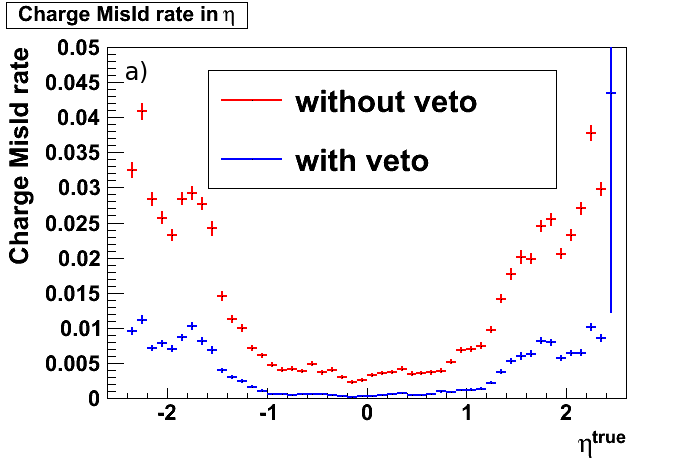
\includegraphics[width=0.485\linewidth,height=0.37\linewidth]{figs/ChargeMisIdRateEta.png}
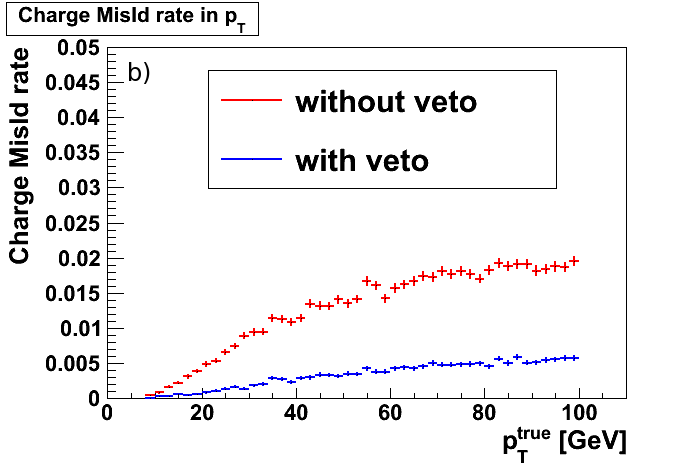
\includegraphics[width=0.485\linewidth,height=0.37\linewidth]{figs/ChargeMisIdRatePt.png}
\caption{Charge mis-identification rate, as a function of a) $\eta$ and b) $p_T$ of the generated
electron using ``electron gun'' sample \label{fig:charge_misid}. The solid (blue) distribution shows
the rate after the veto; if the reconstructed charge is not same for GSF and CTF tracks.}
\end{center}
\end{figure}
Electrons are selected with standard identification and isolation mentioned earlier. The GSF and GeneralTracks 
(CTF) are associated based on sharing of the hits in the silicon strip tracking detector. 
The electrons are vetoed, if the charge of GSF track associated with the electron is not same 
as the charge of the associated GeneralTrack. The electron is considered valid if it has a matched
to a GSF track, but with no associated GeneralTrack. Figure~\ref{fig:charge_misid} shows the charge mis-identification 
rate as a function of pseudorapidity ($\eta$) and transverse momentum ($p_T$) of the generated electron. The charge 
mis-identification rate is reduced by factor of $\sim 3.9$, with a moderate ($2.1\%$)  loss in electron reconstruction 
efficiency after the veto. The rate after the veto is found to vary between $0.04\%$ to $1\%$ with increase in 
pseudorapidity. This selection is applied as part of the standard selection for rest of this document.
